\documentclass[12pt,				% Schriftgroesse
%	pdftex,
	oneside,			% Einseitiger Druck.
	parskip=half,		% Halbe Zeile Abstand zwischen Absätzen.
%	topmargin = 10pt,	% Abstand Seitenrand (Std:1in) zu Kopfzeile [laut log: unused]
	headheight = 12pt,	% Höhe der Kopfzeile
%	headsep = 30pt,	% Abstand zwischen Kopfzeile und Text Body  [laut log: unused]
	headsepline,		% Linie nach Kopfzeile.
	footsepline,		% Linie vor Fusszeile.
	footheight = 16pt,	% Höhe der Fusszeile
	abstracton,		% Abstract Überschriften
	DIV=calc,		% Satzspiegel berechnen
	BCOR=8mm,		% Bindekorrektur links: 8mm
	headinclude=false,	% Kopfzeile nicht in den Satzspiegel einbeziehen
	footinclude=false,	% Fußzeile nicht in den Satzspiegel einbeziehen
	listof=totoc,		% Abbildungs-/ Tabellenverzeichnis im Inhaltsverzeichnis darstellen
	toc=bibliography,	% Literaturverzeichnis im Inhaltsverzeichnis darstellen
]{scrreprt}	% Koma-Script report-Klasse, fuer laengere Bachelorarbeiten alternativ auch: scrbook

\newcommand{\vartitle}{Vorlage für Wissenschaftliche Arbeiten mit LaTeX an der DHBW Horb}
%\vartitle wird außerhalb des dokuments verwendet, womit z.B. \LaTeX, \bf et. nicht funktionieren würden
\newcommand{\vartitleg}{Vorlage für Wissenschaftliche Arbeiten mit \LaTeX\ an der DHBW Horb} 
\newcommand{\varauthor}{Max Musterstudent}
\newcommand{\varsubject}{Besondere Arbeit Nr 1}
\newcommand{\vardhbw}{Stuttgart Campus Horb}
\newcommand{\vardhbwort}{Horb a.~N.}
\newcommand{\varabgabe}{Februärz 2018}
\newcommand{\varabgabedatum}{31. Februärz 2018}
\newcommand{\varmatnr}{1234567}
\newcommand{\varkurs}{TINF2222}
\newcommand{\varfirma}{Musterfirma}
\newcommand{\varfirmaort}{Musterstadt}
\newcommand{\varstudiengang}{Musterstudiengang}
\newcommand{\varbetreuerf}{Max Musterbetreuer}
\newcommand{\varbetreuerh}{Max Musterprofessor}
\newcommand{\vargutachter}{Max Mustergutachter}

\newcommand{\zB}{z.~B. }
\newcommand{\ZB}{Z.~B. }
\errorcontextlines 10000


\usepackage{xstring}
%\usepackage[utf8]{inputenc} % wird von xetex nicht verwendet
\usepackage[T1]{fontenc}
\usepackage{lmodern}
\usepackage[ngerman]{babel}

%%%%%%% Package Includes %%%%%%%
%\usepackage[monochrome]{color} % Einkommentieren für druckversion
\usepackage[margin=2.5cm,foot=1cm]{geometry}	% Seitenränder und Abstände
\usepackage[activate]{microtype} %Zeilenumbruch und mehr
\microtypesetup{expansion=false}
\usepackage[onehalfspacing]{setspace}
\usepackage{makeidx}
\usepackage[autostyle=true,german=quotes]{csquotes}
\usepackage{longtable}
\usepackage{enumitem}	% mehr Optionen bei Aufzählungen
\usepackage{graphicx}
\usepackage{pdfpages}   % zum Einbinden von PDFs
\usepackage{xcolor} 	% für HTML-Notation
\usepackage{float}
\usepackage{array}
\usepackage{calc}		% zum Rechnen (Bildtabelle in Deckblatt)
\usepackage[right]{eurosym}
\usepackage{wrapfig}
\usepackage{pgffor} % für automatische Kapiteldateieinbindung
\usepackage[perpage, hang, multiple, stable]{footmisc} % Fussnoten
\usepackage[printonlyused]{acronym} % falls gewünscht kann die Option footnote eingefügt werden, dann wird die Erklärung nicht inline sondern in einer Fußnote dargestellt
\usepackage{listings}
\usepackage{textcomp}
\usepackage{tikz-cd}
\usepackage{tikz}
\usepackage{tikz-uml}
\usepackage{pgf-pie}
\usepackage{pgfplots}
\usepackage[section]{placeins}
\usepackage{afterpage}
\usepackage{float}
\usepackage[caption = false]{subfig}
\usepackage{mathtools}
\usepackage{forest}
\usepackage{fancyhdr}
\usepackage{lastpage}

\usepackage{blindtext}

% Header und Footer
\pagestyle{headings}
\pagestyle{fancy}
\fancyhead[L]{}
\fancyhead[R]{\textit{\thechapter~\leftmark}}
\fancyfoot{}
\fancyfoot[R]{\thepage}

\fancypagestyle{plain}{%
    \renewcommand{\headrulewidth}{0pt}%
    \fancyhf{}%
    \fancyfoot[R]{\thepage}%
}

\renewcommand{\chaptermark}[1]{\markboth{#1}{}}

\pgfplotsset{compat=1.13}

% Notizen. Einsatz mit \todo{Notiz} oder \todo[inline]{Notiz}. 
\usepackage[obeyFinal,backgroundcolor=yellow,linecolor=black]{todonotes}
% Alle Notizen ausblenden mit der Option "final" in \documentclass[...] oder durch das auskommentieren folgender Zeile
% \usepackage[disable]{todonotes}

% Kommentarumgebung. Einsatz mit \comment{}. Alle Kommentare ausblenden mit dem Auskommentieren der folgenden und dem aktivieren der nächsten Zeile.
%\newcommand{\comment}[1]{\par {\bfseries \color{blue} #1 \par}} %Kommentar anzeigen
% \newcommand{\comment}[1]{} %Kommentar ausblenden

\renewcommand*\rmdefault{lmr}
\fontfamily{lmr}
%%%%%% Configuration %%%%%

%% Anwenden der Einstellungen

% Titel, Autor und Datum
\title{\vartitle}
\author{\varauthor}
%\date{}


% PDF Einstellungen
\usepackage[%
	pdftitle={\vartitle},
	pdfauthor={\varauthor},
	pdfsubject={\varsubject},
	pdfcreator={pdflatex, LaTeX with KOMA-Script},
	pdfpagemode=UseOutlines, 		% Beim Oeffnen Inhaltsverzeichnis anzeigen
	pdfdisplaydoctitle=true, 		% Dokumenttitel statt Dateiname anzeigen.
	pdflang={de_DE}			% Sprache des Dokuments.
]{hyperref}

\definecolor{LinkColor}{HTML}{00007A}
\definecolor{ListingBackground}{HTML}{FCF7DE}

\usepackage[ngerman,nameinlink]{cleveref}

% (Farb-)einstellungen für die Links im PDF
\hypersetup{%
	colorlinks=true, 		% Aktivieren von farbigen Links im Dokument
	linkcolor=LinkColor, 	% Farbe festlegen
	citecolor=LinkColor,
	filecolor=LinkColor,
	menucolor=LinkColor,
	urlcolor=LinkColor,
	linktocpage=true, 		% Nicht der Text sondern die Seitenzahlen in Verzeichnissen klickbar
	bookmarksnumbered=true 	% Überschriftsnummerierung im PDF Inhalt anzeigen.
}
% Workaround um Fehler in Hyperref, muss hier stehen bleiben
\usepackage{bookmark} %nur ein latex-Durchlauf für die Aktualisierung von Verzeichnissen nötig

% Schriftart in Captions etwas kleiner
%\addtokomafont{caption}{\small}

% Literaturverweise (sowohl deutsch als auch englisch)
\usepackage[
	backend=biber,		% empfohlen. Falls biber Probleme macht: bibtex
	bibwarn=true,
	bibencoding=utf8,	% wenn .bib in utf8, sonst ascii
	sortlocale=de_DE,
	style=numeric,
]{biblatex}
\addbibresource{bibliographie.bib}

% Glossar
\usepackage[nonumberlist,toc]{glossaries}



%%%%%% Additional settings %%%%%%

% Hurenkinder und Schusterjungen verhindern
% http://projekte.dante.de/DanteFAQ/Silbentrennung
\clubpenalty = 10000 % schließt Schusterjungen aus (Seitenumbruch nach der ersten Zeile eines neuen Absatzes)
\widowpenalty = 10000 % schließt Hurenkinder aus (die letzte Zeile eines Absatzes steht auf einer neuen Seite)
\displaywidowpenalty=10000

% Bildpfad
\graphicspath{{images/}}

\newcommand\blankpage{%
    \null
    \thispagestyle{empty}%
    \addtocounter{page}{-1}%
    \newpage}

% Einige häufig verwendete Sprachen
\lstloadlanguages{Java}

%Silbentrennung anpassen
\hyphenation{Lauf-fähigkeit}

%Verhindert, dass Akronyme überlang werden
%\renewcommand*\AC@acs[1]{%
%    \expandafter\AC@get\csname fn@#1\endcsname\@firstoftwo{#1}}
%\makeatother

%Begriffdefinition
\newglossaryentry{Training}{
    name=training, 
    description={Sport treiben kann als Training bezeichnet werden}
}
\makeglossaries

\begin{document}

	%!TEX root = ausarbeitung.tex

\begin{titlepage}
	\begin{longtable}{p{8.2cm} p{5.4cm}}
		{\raisebox{\ht\strutbox-\totalheight}{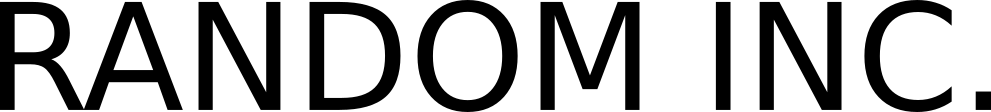
\includegraphics[width=7.8cm,trim=2.5cm 0 0 -1.25cm]{images/randomlogo.png}}} &
		{\raisebox{\ht\strutbox-\totalheight}{
\includegraphics[height=2.2cm,trim=-4cm 0 0 0]{images/dhbw.png}}}
	\end{longtable}
	\enlargethispage{20mm}
	\begin{center}
		\vspace*{12mm}	{\LARGE\textbf \vartitleg }\\
		\vspace*{12mm}	{\large\textbf \varsubject }\\
		%\vspace*{12mm}	\langdeckblattabschlusshinleitung\\
		%\vspace*{3mm}		{\textbf \abschluss}\\
		\vspace*{12mm}	des Studiengangs \varstudiengang \\
    \vspace*{3mm}		an der \\ Dualen Hochschule Baden-Württemberg \\ \vardhbw \\
		\vspace*{12mm}	von \\
		\vspace*{3mm}		{\large\textbf \varauthor}\\
		\vspace*{12mm}	\varabgabe \\
	\end{center}
	\vfill
	\begin{spacing}{1.2}
	\begin{tabbing}
		mmmmmmmmmmmmmmmmmmmmmmm             \= \kill
		\textbf{Matrikelnummer, Kurs}  \>  \varmatnr, \varkurs \\
		\textbf{Firma}                  \>  \varfirma, \varfirmaort \\
		\textbf{Betreuer der Firma}               \>  \varbetreuerf \\
		\textbf{Betreuer der Hochschule}               \>  \varbetreuerh \\
		%\textbf{Gutachter}              \>  \vargutachter
	\end{tabbing}
	\end{spacing}
\end{titlepage}
%\blankpage
	\pagenumbering{Roman}
	%!TEX root = ausarbeitung.tex

\thispagestyle{empty}
\addchap{Eidesstattliche Erklärung}
%\chapter*{Eidesstattliche Erklärung}
% http://www.se.dhbw-mannheim.de/fileadmin/ms/wi/dl_swm/dhbw-ma-wi-organisation-bewertung-bachelorarbeit-v2-00.pdf
\vspace*{2em}

Ich versichere hiermit, dass ich meine {\varsubject} mit dem Thema: {\itshape \vartitle } selbstständig verfasst und keine anderen als die angegebenen Quellen und Hilfsmittel benutzt habe. Ich versichere zudem, dass die eingereichte elektronische Fassung mit der gedruckten Fassung übereinstimmt. 

% https://www.dhbw-karlsruhe.de/fileadmin/user_upload/dokumente/T-Informatik/Prüfungsordnung-Technik-2015-09-29.pdf (S. 19)


% Ich erkläre hiermit ehrenwörtlich: \\
% \begin{enumerate}
% \item dass ich meine {\arbeit} mit dem Thema
% {\itshape \titel } ohne fremde Hilfe angefertigt habe;
% \item dass ich die Übernahme wörtlicher Zitate aus der Literatur sowie die Verwendung der Gedanken
% anderer Autoren an den entsprechenden Stellen innerhalb der Arbeit gekennzeichnet habe;
% \item dass ich meine {\arbeit} bei keiner anderen Prüfung vorgelegt habe;
% \item dass die eingereichte elektronische Fassung exakt mit der eingereichten schriftlichen Fassung
% übereinstimmt.
% \end{enumerate}
% 
% Ich bin mir bewusst, dass eine falsche Erklärung rechtliche Folgen haben wird.

% % http://www.ib.dhbw-mannheim.de/fileadmin/ms/bwl-ib/Downloads_alt/Leitfaden_31.05.pdf (S. 52)



\vspace{3em}

\vardhbwort, \varabgabedatum
\vspace{4em}

\rule{6cm}{0.4pt}\\
\varauthor

	
	%!TEX root = ausarbeitung.tex

\addchap{Abkürzungsverzeichnis}
%nur verwendete Akronyme werden letztlich im Abkürzungsverzeichnis des Dokuments angezeigt
%Verwendung: 
%		\ac{Abk.}   --> fügt die Abkürzung ein, beim ersten Aufruf wird zusätzlich automatisch die ausgeschriebene Version davor eingefügt bzw. in einer Fußnote (hierfür muss in header.tex \usepackage[printonlyused,footnote]{acronym} stehen) dargestellt
%		\acs{Abk.}   -->  fügt die Abkürzung ein
%		\acf{Abk.}   --> fügt die Abkürzung UND die Erklärung ein
%		\acl{Abk.}   --> fügt nur die Erklärung ein
%		\acp{Abk.}  --> gibt Plural aus (angefügtes 's'); das zusätzliche 'p' funktioniert auch bei obigen Befehlen
%	siehe auch: http://golatex.de/wiki/%5Cacronym
%	
\begin{acronym}[YTMMM]
\setlength{\itemsep}{-\parsep}

\acro{AGPL}{Affero GNU General Public License}
\end{acronym}


	\printglossaries
	
	\listoffigures

	%\listoftables

	% Inhaltsverzeichnis
	\begin{spacing}{1.1}
		\setcounter{tocdepth}{1}
		\renewcommand*{\chapterpagestyle}{empty}
		\tableofcontents
		\clearpage
	\end{spacing}

	\pagenumbering{arabic}

	% Inhalt
	\foreach \i in {01,02,03,04,05,06,07,08,09,...,99} {%
		\edef\FileName{content/\i kapitel}%
			\IfFileExists{\FileName}{%
				\input{\FileName}
			}
			{%
				%file does not exist
			}
	}

	%\nocite{*}
	\printbibliography

\end{document}